\documentclass[conference]{IEEEtran}
\usepackage{amsmath,amssymb}
\usepackage{booktabs}
\usepackage{url}
\usepackage{array}
\usepackage{graphicx}
\usepackage{placeins}
\setlength{\textfloatsep}{9pt plus 2pt minus 3pt}
\setlength{\floatsep}{8pt plus 2pt minus 2pt}
\setlength{\intextsep}{8pt plus 2pt minus 2pt}

\title{Historical Group Risk for Budget-Constrained SSD Maintenance Prioritisation}

\author{
\begin{tabular}{ccc}
\begin{tabular}{c}Sumedh Udupa U\\Department of Computer Science\\R. V. College of Engineering\\Bengaluru-560059, India\\sumedhu.cs23@rvce.edu.in\end{tabular} &
\begin{tabular}{c}Syed Muzammil Hussaini\\Department of Computer Science\\R. V. College of Engineering\\Bengaluru-560059, India\\syedmuzammilh.cs23@rvce.edu.in\end{tabular} &
\begin{tabular}{c}Varun Gowda R\\Department of Computer Science\\R. V. College of Engineering\\Bengaluru-560059, India\\varungowdar.cs23@rvce.edu.in\end{tabular}
\end{tabular}\\[1.0em]
\begin{tabular}{c}
Prapulla S. B.\\Department of Computer Science\\R. V. College of Engineering\\Bengaluru-560059, India\\prapullasb@rvce.edu.in
\end{tabular}
}

\begin{document}
\maketitle

\begin{abstract}
Data-centre operators must decide which devices to inspect or replace when
maintenance capacity is limited. We study a transparent decision-support method that
uses historical failure rates for SSD models and racks to rank eligible drives under
an explicit device-count budget. The primary ranking uses failure tickets, fleet
inventory, and rack assignments; it does not use SMART attributes. Using the Alibaba
SSD reliability dataset, we compare
model-aware, rack-aware, and weighted multi-factor rankings with random selection in
a chronological evaluation at four decision dates and four budgets. Across the four
dates, the rack-aware strategy captures a mean 18.7\% of subsequent failures at a 5\%
budget (3.74$\times$ mean lift over random). At a 20\% budget, the multi-factor
strategy with model weight 0.3 captures a mean 60.4\% of subsequent failures (3.02$\times$
mean lift). In a separate temporal SMART holdout over six mapped model families,
LightGBM captures 21.6\% of test failures at 5\% capacity (4.32$\times$ lift) and
63.4\% at 20\% (3.17$\times$), on the same 373,511-drive test cohort as DRIVE.
These are retrospective ranking results, not individual failure probabilities or
causal estimates of maintenance benefit. The SMART result is limited to one temporal
split and six model families; it does not replace the separate full-fleet
evaluation or establish performance on other fleets.
\end{abstract}

\begin{IEEEkeywords}
SSD reliability, maintenance prioritisation, data centres, failure analysis,
resource allocation, explainability
\end{IEEEkeywords}

\section{Introduction}
Storage operators manage large fleets whose failures are not evenly distributed
across device models and physical infrastructure. Prior field studies describe SSD
failure characteristics and spatial correlations at scale~\cite{maneas2020,han2021}.
Prediction work also uses device telemetry to estimate drive-level failure risk~\cite{lu2020}.
Yet a maintenance team must still convert evidence into a finite inspection or
replacement list. That step has a capacity constraint: only a fraction of the fleet can
be handled during one maintenance cycle.

This paper evaluates a simple decision-support approach that ranks eligible drives
using historical failure rates for their model and rack. It asks: under the same
maintenance-capacity budget, do infrastructure-aware and multi-factor rankings capture
more subsequent failures than model-aware or random selection? The contribution is an
equal-budget, chronological comparison of interpretable group-risk rankings on one
large SSD fleet. The work is not an individual-drive failure predictor: the score
assigned to a drive is derived from its group's past failures.

\section{Related Work}
Large-scale studies have documented failure patterns in hard drives and SSDs, including
the reliability of enterprise deployments~\cite{pinheiro2007,maneas2020} and correlated
failures in production SSD racks and nodes~\cite{han2021}. Other work investigates
telemetry-based failure prediction~\cite{lu2020}; operational SSD studies also examine
fail-stop and fail-slow behavior~\cite{lu2022}. These studies establish the importance
of both device signals and infrastructure context. Our method addresses a narrower question:
how historical model- and rack-level rates behave as an explainable ranking when the
number of selected drives is fixed. We make no priority claim that this is the first
such method.

\section{Data and Methods}
\subsection{Primary Fleet Data and Cohort}
The analysis uses the Alibaba SSD failure tickets and location records released with
the production reliability study~\cite{han2021}. Device identity is the pair
$(\text{model},\text{disk\_id})$, since disk identifiers repeat across model namespaces.
The primary cohort is reconstructed from the location inventory and failure tags. The
local SMART file is a separate one-day snapshot; its attribute values are not used to
build the historical group-risk scores. The records contain 965,495 unique drives,
18,387 failure events, and 11 models over the 2018--2019 observation interval. The
full-fleet evaluation uses
decision dates 2019-01-01, 2019-04-01, 2019-07-01, and 2019-10-01. For each date $t$,
history uses events strictly before $t$, and outcomes are failures strictly after $t$
through 2019-12-31. The four outcome windows overlap and are not independent
replications. Their failure counts are 12,143, 10,124, 7,239, and 3,104, respectively.

\subsection{Historical Group-Risk Scores}
For a group with $k$ observed failures and $E$ accumulated drive-days, we use a
Gamma--Poisson posterior mean shrunk toward a parent rate $\theta_p$:
\begin{equation}
 \widehat{\lambda}=\frac{k+\beta\theta_p}{E+\beta},\qquad \beta=730\text{ drive-days}.
\end{equation}
Model rates shrink toward the fleet rate. Rack rates are estimated within model and
shrink toward that model's rate. Per-drive deployment dates are unavailable, so the
primary exposure estimate assumes a static fleet over the two-year observation window;
failed drives contribute exposure through their failure day. At each decision date,
event counts, exposure, and parent rates are recomputed from the history available
strictly before that date.
Drive-level scores are therefore group rates; they are not calibrated probabilities
that a particular drive will fail.

\subsection{Ranking Strategies and Capacity Budgets}
The comparison includes random, model-aware, infrastructure-aware, and multi-factor
strategies. The multi-factor score is
\begin{equation}
 S(d)=wR_m(d)+(1-w)R_r(d),\quad w\in\{0.7,0.5,0.3\},
\end{equation}
where $R_m$ and $R_r$ are min--max normalised model and model--rack historical rates.
For budget $B\in\{5,10,15,20\}\%$, each strategy selects
$K=\lfloor BN/100\rfloor$ drives from its eligible population. Deterministic
tie-breaking uses model and drive identifier; random selection is repeated for 100
seeds (0--99). Selected records have explanatory strings identifying the group rates
that determined their rank. The eligibility rule excludes drives with a known failure
strictly before $t$; failure-at-$t$ drives remain eligible. All drives in this dataset
have rack assignments, so every strategy has the same eligible population and $K$.

\subsection{Evaluation Metrics}
Failure coverage is the fraction of subsequent failures in the selected set. Precision
is the fraction of selected drives that fail in the outcome window. Lift is coverage
divided by the selected budget share. For the headline table, each metric is calculated
for each decision date and then averaged arithmetically over the four dates. Random
values are the mean of 100 draws per date and budget. The four date-specific evaluation
windows share later calendar periods. Accordingly, date averages are descriptive
summaries rather than independent-sample estimates; we do not report significance tests
or interpret the four dates as independent trials.
The mean random lift is 1.000--1.001 across dates. Mean within-date standard deviation
across the 100 random draws is 0.054, 0.037, 0.031, and 0.025 at 5\%, 10\%, 15\%, and
20\% budgets, respectively.

\subsection{Separate Temporal SMART Evaluation}
We also compare DRIVE rankings with the Alibaba Tianchi 95044 daily telemetry release
for six mapped model families~\cite{xu2021}. The published model crosswalk was checked
against the primary failure tickets; all 16,305 events in the matched families agree
by model, drive identifier, and timestamp. The training cohort uses SMART attributes
recorded on 2019-07-01 and failures in the following quarter (380,907 eligible drives;
3,550 failed-drive keys across 3,845 events). The held-out cohort uses attributes
recorded on 2019-10-01 and failures in the next quarter (373,511 eligible drives;
2,716 failed-drive keys across 2,913 events). All held-out drives join to the primary
location inventory and rack pool.

The SMART threshold ranks the number of positive raw counters among attributes 5,
187, 196, 197, and 198. Logistic regression and LightGBM use numeric SMART attributes
and model indicators. Fifty-six nonempty, nonconstant attributes are selected using
training features only; imputation, scaling, class weighting, and model fitting use
training data only. Configuration is fixed before evaluation on the held-out cohort.
DRIVE scores use failure history strictly before 2019-10-01 and rank the same held-out
drives. No held-out positive drive key was a training-period failure. Some surviving
drives occur in both cohorts, so this is a temporal evaluation rather than a
drive-disjoint split. This comparison does not replace or alter the full-fleet
evaluation above.

\section{Experimental Results}
\subsection{Full-Fleet Historical Ranking}
Table~\ref{tab:headline} reports means across the four decision dates. At 5\%,
infrastructure-aware selection has the highest lift (3.74$\times$) and covers 18.7\%
of subsequent failures on average. Figure~\ref{fig:full-fleet-coverage} shows coverage
over all tested budgets: the rack-risk ranking leads at 5\%, while the multi-factor
strategy with $w=0.3$
has the highest mean lift among the tested risk rankings (3.02$\times$) and covers
60.4\%. The random baseline has mean lift approximately one, as expected under the
metric definition.

\begin{table}[t]
\caption{Mean full-fleet results over four decision dates. Coverage and precision are fractions.}
\label{tab:headline}
\centering
\small
\begin{tabular}{llrrr}
\toprule
Strategy & $w$ & Budget & Lift & Coverage \\
\midrule
Random & -- & 5\% & 1.00 & 0.050 \\
Model & -- & 5\% & 1.34 & 0.067 \\
Rack & -- & 5\% & \textbf{3.74} & \textbf{0.187} \\
Multi & 0.7 & 5\% & 1.77 & 0.088 \\
Multi & 0.5 & 5\% & 1.82 & 0.091 \\
Multi & 0.3 & 5\% & 2.62 & 0.131 \\
\midrule
Random & -- & 20\% & 1.00 & 0.200 \\
Model & -- & 20\% & 2.55 & 0.510 \\
Rack & -- & 20\% & 2.85 & 0.571 \\
Multi & 0.7 & 20\% & 2.98 & 0.597 \\
Multi & 0.5 & 20\% & 2.99 & 0.597 \\
Multi & 0.3 & 20\% & \textbf{3.02} & \textbf{0.604} \\
\bottomrule
\end{tabular}
\end{table}

\begin{figure}[!t]
\centering
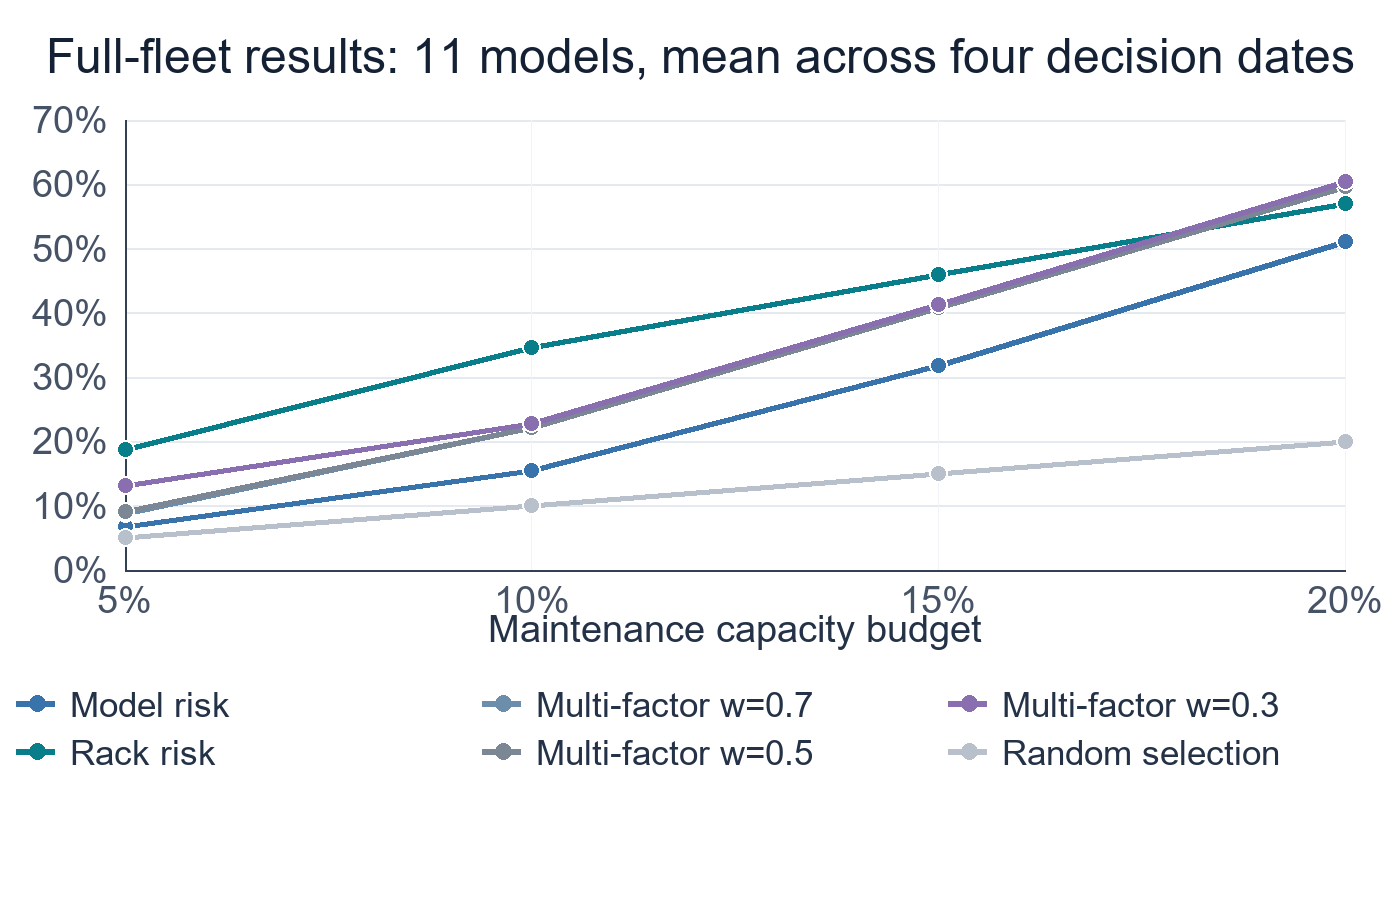
\includegraphics[width=\linewidth]{figures/full_fleet_coverage.png}
\caption{Failure coverage across budgets in the full 11-model fleet, averaged over four
decision dates. All tested historical rankings are shown.}
\label{fig:full-fleet-coverage}
\end{figure}

The best strategy depends on capacity: rack-level risk is most effective at the
tightest evaluated budget, while the multi-factor ranking with greater rack emphasis
performs best at 20\%. The supplementary full-fleet result table contains the complete
strategy-by-budget grid.

We also reran the complete grid under a snapshot-anchored exposure bound. In this
sensitivity analysis, drives absent from the final SMART snapshot contribute zero
exposure while still healthy at the decision date. This assumption uses future
end-state presence and is not available to an operator at decision time; it is reported
only as a retrospective bound. The winning broad strategy is unchanged at each budget,
but the 20\% multi-factor winner changes from $w=0.3$ to $w=0.7$. Across strategy and
budget cells, primary and sensitivity mean lifts have Spearman correlation 0.832, while
mean coverage has correlation 0.965. The reductions in absolute lift and coverage show
that effect sizes are sensitive to the missing deployment-tenure information.
Table~\ref{tab:exposure-sensitivity} reports the primary and sensitivity winners and
their four-date mean scores at each budget.

\begin{table*}[t]
\caption{Primary and snapshot-anchored sensitivity results for the best risk ranking at each budget. The sensitivity uses end-of-window snapshot presence and is not a decision-time estimate.}
\label{tab:exposure-sensitivity}
\centering
\small
\begin{tabular}{rlrrlrr}
\toprule
Budget & Primary winner & Lift & Coverage & Sensitivity winner & Lift & Coverage \\
\midrule
5\%  & Rack & 3.74 & 18.7\% & Rack & 2.56 & 12.8\% \\
10\% & Rack & 3.46 & 34.6\% & Rack & 2.68 & 26.8\% \\
15\% & Rack & 3.06 & 45.9\% & Rack & 2.69 & 40.4\% \\
20\% & Multi ($w=0.3$) & 3.02 & 60.4\% & Multi ($w=0.7$) & 2.80 & 56.0\% \\
\bottomrule
\end{tabular}
\end{table*}

\subsection{Temporal Telemetry Comparison}
Table~\ref{tab:telemetry} summarizes selected capacity budgets on the matched temporal
cohort. LightGBM has the highest coverage at both reported budgets. DRIVE's
infrastructure ranking is below LightGBM in this telemetry comparison, although it
captures 58.25\% of held-out failures at 20\% capacity. Random intervals describe
variation across 100 selection seeds, not uncertainty across fleets or years. This
result is limited to one historical split and six model families. Figure~\ref{fig:temporal-smart-coverage}
shows coverage across all four budgets for every evaluated ranking.

\begin{table*}[t]
\caption{Metrics on the six-family October temporal test cohort (373,511 eligible drives; 2,716 failed drives). Random intervals are empirical 2.5th--97.5th seed percentiles.}
\label{tab:telemetry}
\centering
\small
\begin{tabular}{lrrrr}
\toprule
Strategy & Coverage @5\% & Lift @5\% & Coverage @20\% & Lift @20\% \\
\midrule
Random & 5.05\% (4.40--5.87) & 1.009 (0.880--1.175) & 20.05\% (18.80--21.54) & 1.002 (0.940--1.077) \\
SMART threshold & 15.72\% & 3.144 & 28.65\% & 1.432 \\
Logistic regression & 19.26\% & 3.851 & 57.92\% & 2.896 \\
LightGBM & 21.58\% & 4.315 & 63.40\% & 3.170 \\
DRIVE model & 3.57\% & 0.714 & 31.11\% & 1.556 \\
DRIVE infrastructure & 16.02\% & 3.203 & 58.25\% & 2.912 \\
DRIVE multi ($w=0.7$) & 5.41\% & 1.083 & 53.65\% & 2.682 \\
DRIVE multi ($w=0.5$) & 11.52\% & 2.305 & 53.76\% & 2.688 \\
DRIVE multi ($w=0.3$) & 14.95\% & 2.990 & 53.28\% & 2.664 \\
\bottomrule
\end{tabular}
\end{table*}

\begin{figure}[!t]
\centering
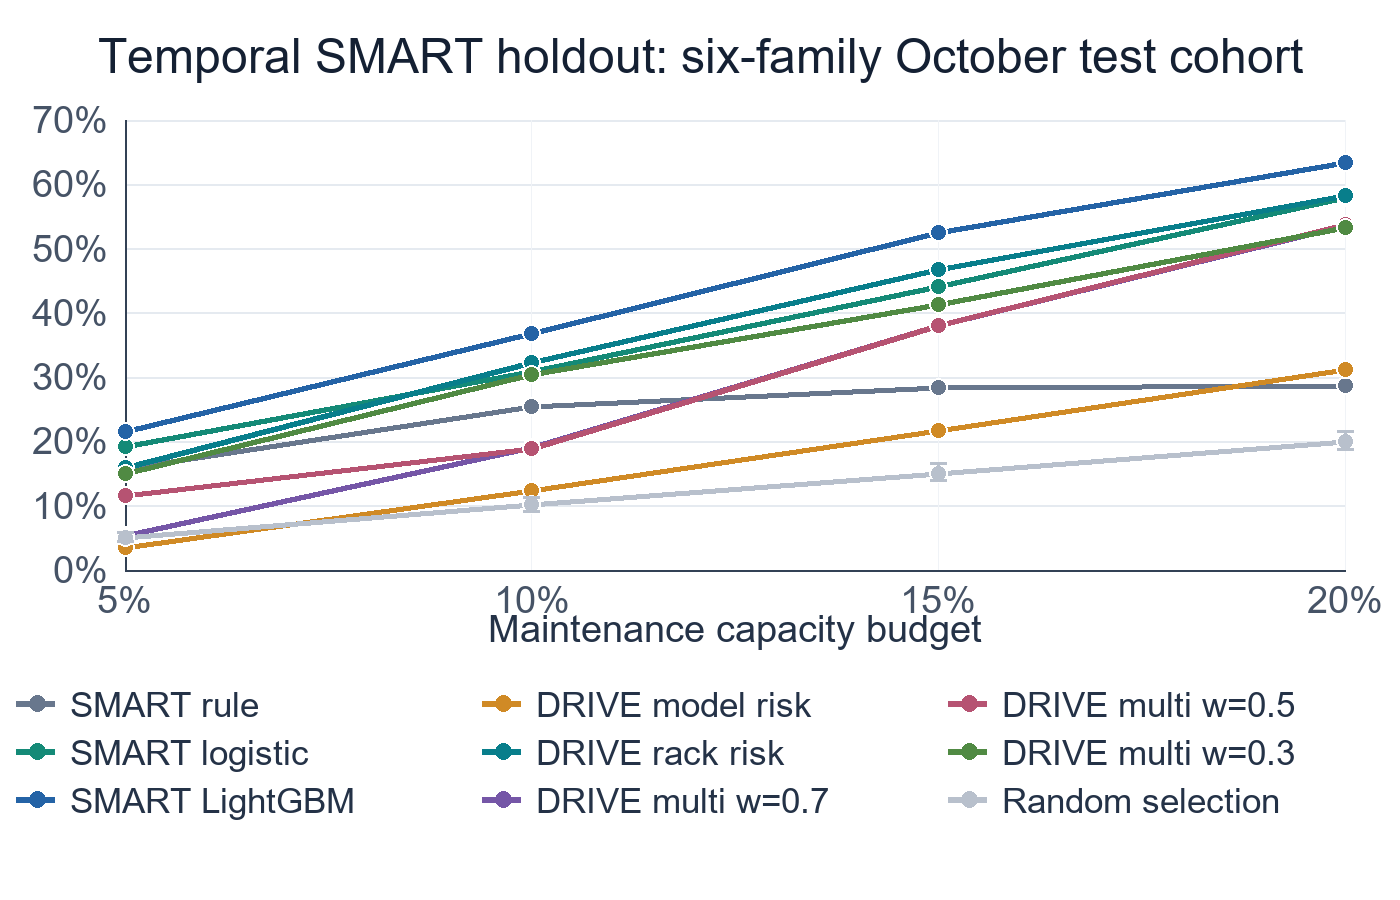
\includegraphics[width=\linewidth]{figures/temporal_smart_coverage.png}
\caption{Failure coverage versus capacity in the six-family temporal SMART holdout.
All SMART and DRIVE rankings are shown. Error bars on random selection are the
2.5th--97.5th percentiles across 100 seeds; they describe seed variability only.}
\label{fig:temporal-smart-coverage}
\end{figure}

\subsection{Illustrative Selection Explanation}
At the 2019-07-01 decision date and 5\% budget, the highest-ranked rack example is
drive (A3, 35691) in rack 18670. Its model and rack rates are historical group rates
available at that date. The multi-factor score combines their normalized values, and
the explanation exposes both components. These values justify the rank under the
specified rule; they are not an estimate of that drive's individual failure probability.

\begin{table}[t]
\caption{Computed rank-1 examples at 2019-07-01, 5\% budget. Rates are per drive-day.}
\label{tab:explanation-example}
\centering
\scriptsize
\begin{tabular}{p{1.5cm}p{1.7cm}p{3.1cm}r}
\toprule
Strategy & Drive & Group evidence & Score \\
\midrule
Model & C2 / 0 & Model rate $6.966\times10^{-5}$; norm 1.000 & 1.000 \\
Rack & A3 / 35691 & Rack 18670 rate $2.996\times10^{-3}$; norm 1.000 & 1.000 \\
Multi $w=0.3$ & A3 / 35691 & Model $5.859\times10^{-5}$ (norm 0.832); rack $2.996\times10^{-3}$ (norm 1.000) & 0.950 \\
\bottomrule
\end{tabular}
\end{table}

\section{Discussion}
On the full fleet, rack history is most useful at tight capacity, while the multi-factor
ranking with greater rack emphasis performs best among the tested historical rankings
at 20\%. In the separate telemetry cohort, LightGBM captures more test failures than
DRIVE at both reported budgets. These results come from one historical split on six
model families, not evidence of broad superiority across fleets or years. Neither
ranking establishes that maintenance based on its list prevents failures, reduces
cost, or improves future fleet reliability.

The design is intentionally interpretable: each choice can be traced to a model or
rack group's past rate. This makes the ranking inspectable, but it also means that
drives sharing a group receive similar group-risk signals. The score should be used
for prioritisation or investigation, not as an individual failure probability.

\section{Limitations and Future Work}
First, the study is retrospective and uses one operator's records from 2018--2019. The
telemetry comparison contains one temporal split and six mapped model families; 351,144 drive keys appear
in both eligible time cohorts, so the results do not represent an independent-drive
holdout. Second, failure-table absence is treated as no recorded failure in the window,
not proof of health, and unrecorded removals can affect labels. Third, the telemetry
models' class-weighted ranking scores are not calibrated probabilities. Fourth, the
historical group-rate
estimator assumes static exposure over parts of the observation period; reported rates
are not calibrated time-varying hazards. Fifth, results depend on group definitions,
smoothing strength, and the tested multi-factor weights. Maintenance costs and
intervention outcomes are absent, so budgets represent drive-count capacity rather
than monetary cost. Evaluation on additional fleets and periods, improved censoring
information, and intervention studies remain future work.

\FloatBarrier
\section{Conclusion}
We compared chronological model-, rack-, and multi-factor historical group-risk
rankings under equal drive-count budgets and evaluated them separately against SMART
methods on a common six-family temporal cohort. In the full 11-model fleet, rack-aware
selection achieves a 3.74$\times$ mean lift at 5\%, while the $w=0.3$ multi-factor
ranking achieves a 3.02$\times$ mean lift at 20\%. On the telemetry cohort, LightGBM captures 21.58\% of test failures at 5\% and 63.40\%
at 20\%, while DRIVE infrastructure selection captures 16.02\% and 58.25\%,
respectively. These results support transparent group-risk ranking as a decision aid,
while showing that telemetry can improve selection in the tested subset. They do not
establish individual failure probabilities, broad generalization, or maintenance
benefit.

\bibliographystyle{IEEEtran}
\bibliography{references}
\end{document}
